\documentclass[../slides.tex]{subfiles}
\begin{document}

\begin{frame}{Datenerfassung}
  
\begin{minipage}[t]{.3\textwidth}
    \begin{block}{Photogammetry}
        \begin{itemize}
            \item Geringe Einstiegskosten
            \item Wenig Größenlimits
            \item Auflösung Situationsabhänig
            \item Skaliert mit Arbeitsaufwand
            \item Genauigkeit im cm-Bereich
        \end{itemize}
    \end{block}
    \end{minipage}
    \hfill
    \begin{minipage}[t]{.69\textwidth}
    \begin{figure}[]
        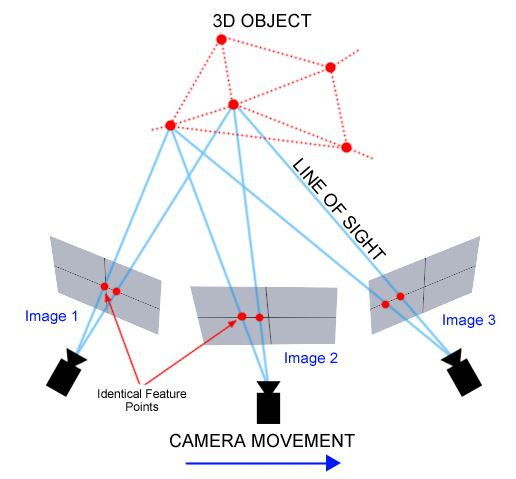
\includegraphics[height=150pt]{img_niklas/photogrammetry.jpg}
        \caption{}
        \label{fig:photogrammetry}
    \end{figure}
    \end{minipage}
    
\end{frame}

\begin{frame}{Datenerfassung}
    \begin{minipage}[t]{.5\textwidth}
        \begin{block}{Laserscanning}
            \begin{itemize}
                \item Hohe Auflösung
                \item Kostenfaktor
                \item Bauteilgröße limitert
                \item Genauigkeit im $\mu$ m-Bereich
            \end{itemize}
        \end{block}
        \end{minipage}
        \hfill
        \begin{minipage}[t]{.49\textwidth}
        \begin{figure}[]
            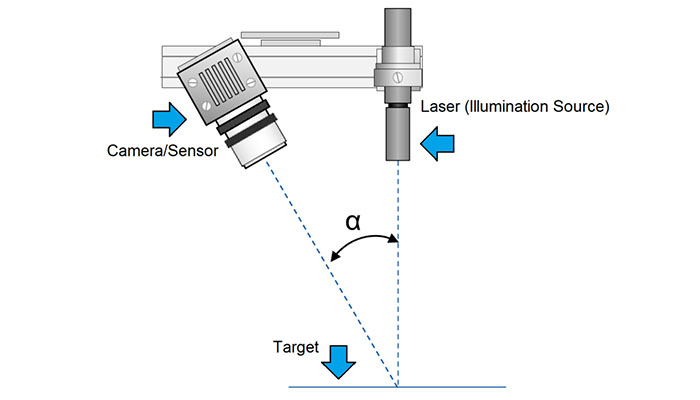
\includegraphics[height=150pt]{img_niklas/laser_1.jpg}
            \caption{}
            \label{fig:laserscanner}
        \end{figure}
        \end{minipage}
    \end{frame}

\begin{frame}{Datenerfassung: Versuchsaufaufbau}
    \begin{minipage}[t]{.3\textwidth}
        \begin{itemize}
            \item 1: Schraubstockbacken
            \item 2: Demonstratorbauteil
            \item 3: Scannerhalterung
            \item 4: Scanner
            \item 5: Verschiebungsmesser
            \item 6: Schraubstock
            \item 7: Laserlinie
        \end{itemize}
        \end{minipage}
        \hfill
        \begin{minipage}[t]{.65\textwidth}
        \begin{figure}[]
            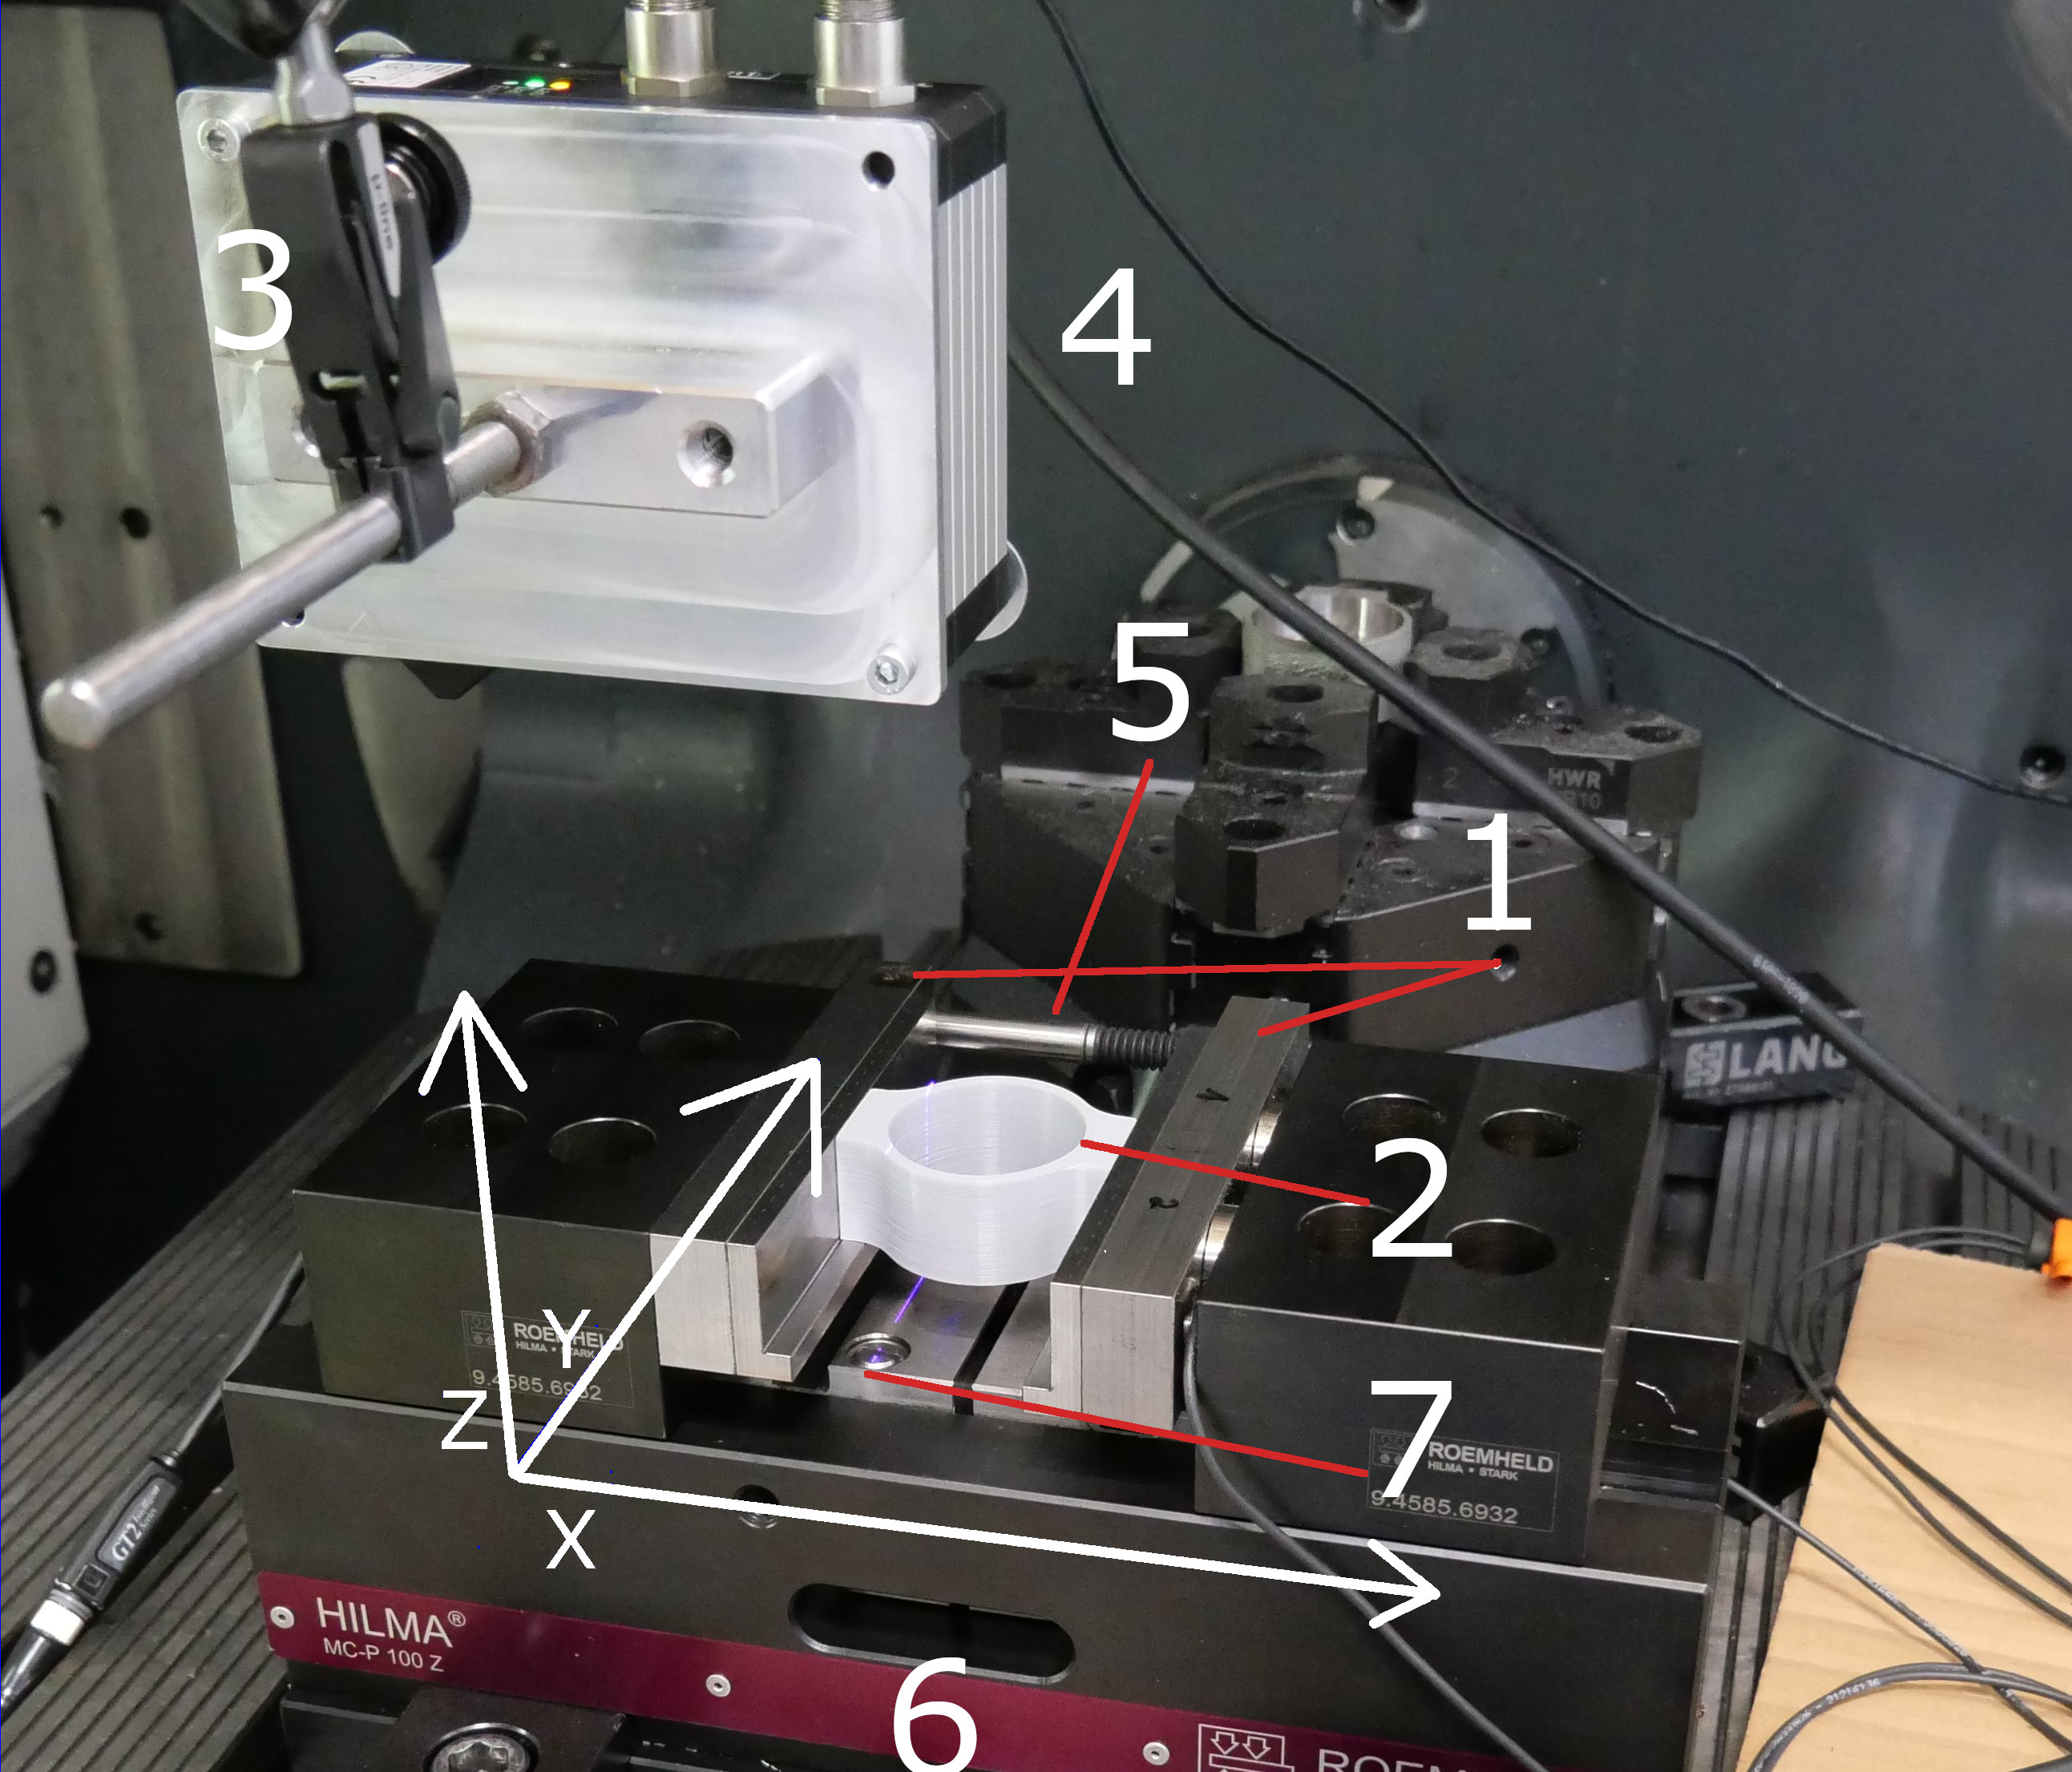
\includegraphics[height=150pt]{img_niklas/versuchsaufbau_foto.png.JPG}
            \caption{Versuchsaufaufbau}
            \label{fig:versuchsaufbau}
        \end{figure}
        \end{minipage}
\end{frame}

\begin{frame}{Datenerfassung: Laser-Linienmesser}
    \begin{minipage}[t]{.3\textwidth}
        \begin{figure}[]
            \centering
            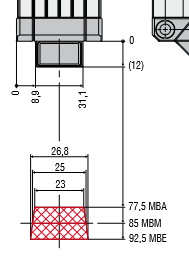
\includegraphics[height=150pt]{img_niklas/Scanner.PNG}
            \caption{Laser-Linienmesser}
            \label{fig:linescanner}
        \end{figure}
        \end{minipage}
        \hfill
        \begin{minipage}[t]{.65\textwidth}
        \begin{figure}[]
            \centering
            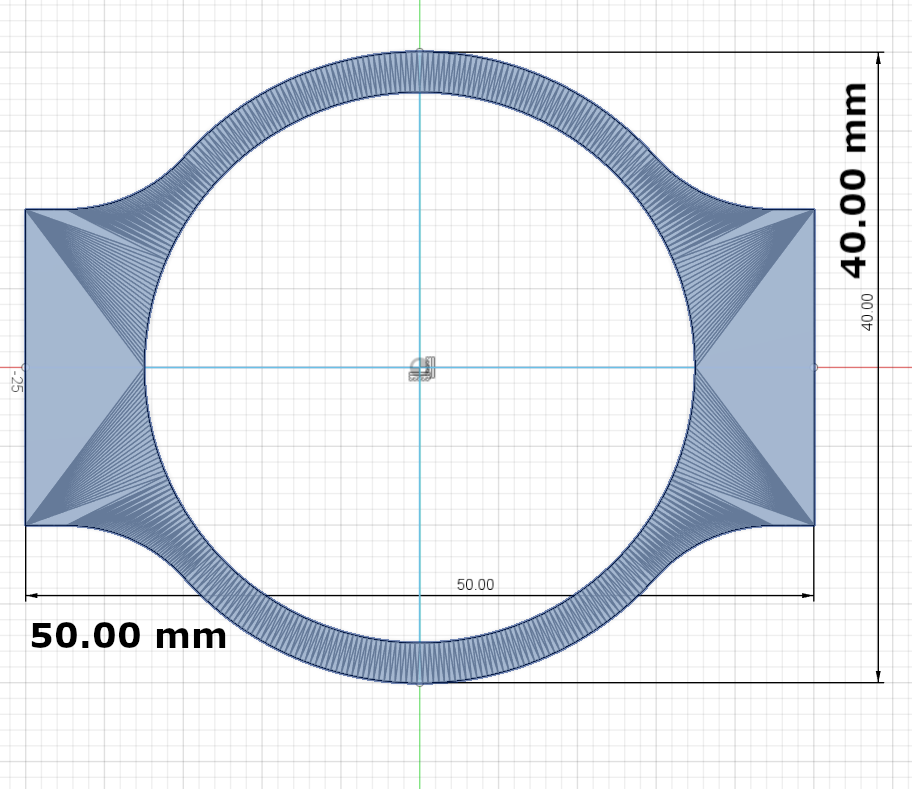
\includegraphics[height=150pt]{img_niklas/demo_size.png}
            \caption{Bemaßtes Demonstratorbauteil}
            \label{fig:versuchsaufbau}
        \end{figure}
        \end{minipage}
\end{frame}

\begin{frame}{Datenerfassung: Scanergebnis}
    \begin{figure}
        \centering
        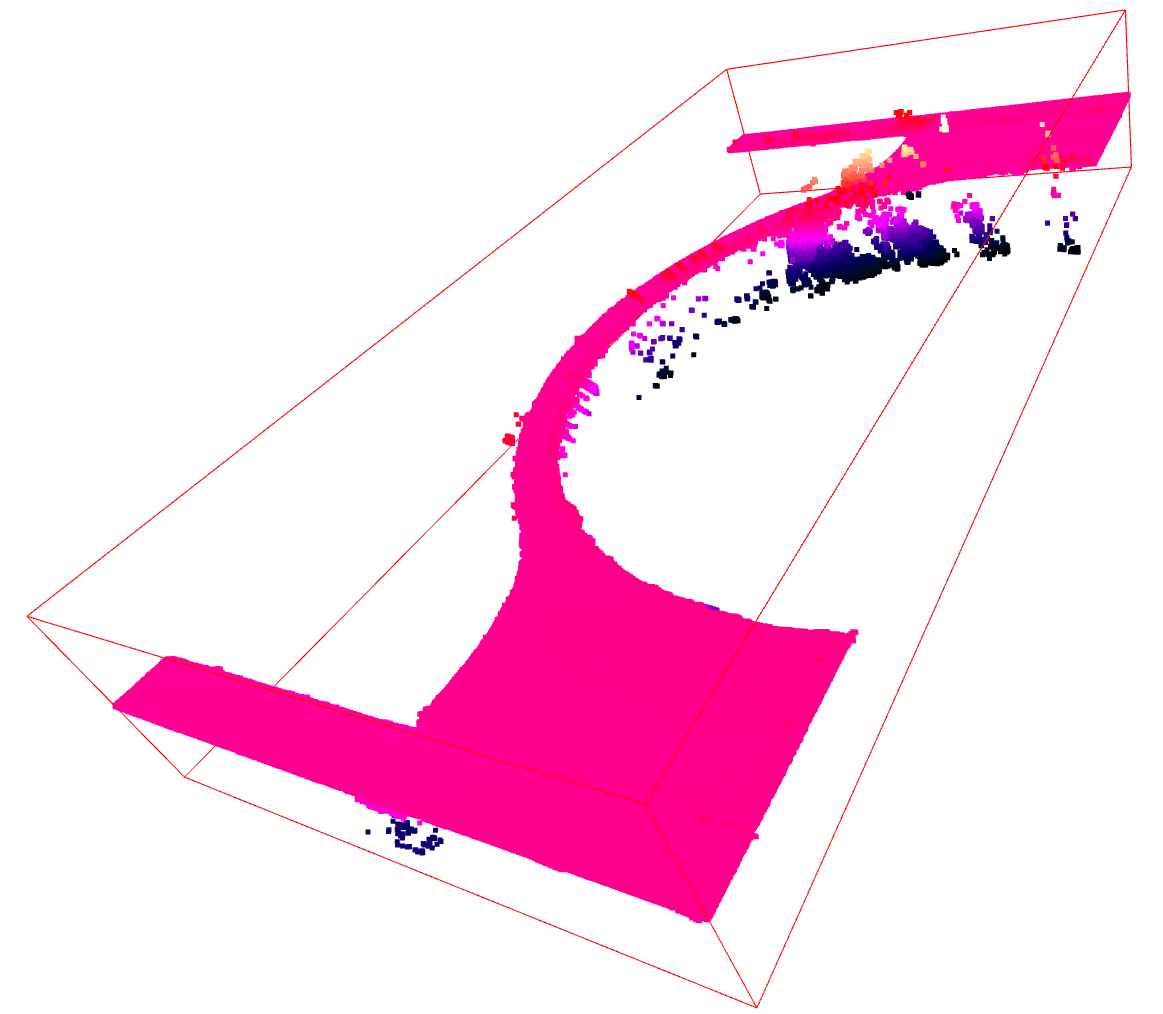
\includegraphics[height=150pt]{img_niklas/pc_with_outliers.PNG}
        \caption{Pointcloud}
        \label{fig:pcoultiers}
    \end{figure}
\end{frame}


\end{document}